\documentclass[a4paper,10pt]{jsarticle}

% レイアウト
\setlength{\textwidth}{\fullwidth}
\setlength{\textheight}{39\baselineskip}
\addtolength{\textheight}{\topskip}
\setlength{\voffset}{-0.5in}
\setlength{\headsep}{0.3in}
\pagestyle{myheadings}

% パッケージ
\usepackage[dvipdfmx]{graphicx}
\usepackage{amsmath,amssymb,epsfig}
\usepackage{bm}
\usepackage{ascmac}
\usepackage{pifont}
\usepackage{multirow}
\usepackage{enumerate}
\usepackage{cases}
\usepackage{type1cm}
\usepackage{cancel}
\usepackage{url}
\usepackage{listings,jlisting}
% 大きな中括弧
\usepackage{cases}

% 定義
\DeclareMathOperator*{\argmin}{arg\,min}
\DeclareMathOperator*{\argmax}{arg\,max}
\def\vec#1{\mbox{\boldmath$#1$}}
\def\R{{\Bbb R}}

% カウンタの設定
\setcounter{section}{0}
\setcounter{subsection}{0}
\setcounter{subsubsection}{0}
\setcounter{equation}{0}

% キャプションの図をFigに変更
\renewcommand{\figurename}{Fig.}
\renewcommand{\tablename}{Tab.}

% 式番号を式(章番号.番号)に
\makeatletter
\renewcommand{\theequation}{\arabic{section}.\arabic{equation}}
\@addtoreset{equation}{section}
\makeatother

% 表紙
\title{知能システム学特論レポート}
\author{
(DL2班)Caffe on Ubuntu\\
}
\date{2015年\ 6月\ 29日}

% ドキュメントの開始
\begin{document}
\maketitle
\section{報告者}
\begin{list}{}{}
 \item 15344203\hspace{0.5cm} 有田 裕太
 \item 15344206\hspace{0.5cm} 緒形 裕太
 \item 15344209\hspace{0.5cm} 株丹 亮
 \item 12104125\hspace{0.5cm} 宮本 和
\end{list}

\section{進行状況}

\begin{itemize}
\item 理論研究
\item 順伝播型ネットワークについて
\end{itemize}

\section{理論研究}
\subsection{単純型細胞と複雑型細胞}
単純型細胞と複雑型細胞のモデルをFig.~\ref{fig:単純型細胞と複雑型細胞の
モデル}に示す.(a),(b)は4×4の入力層が中間層のそれぞれと結合していること
を示しており,(c),(d)は入力パターンの位置変化に伴う中間層および出力層の
状態の変化を示している.

中間層は単純型細胞,出力層は複雑型細胞のモデルと
なっており,中間層は位置選択性が厳密であるが,出力層は入力パターンが少し
ずれても活性化する.全体への入力が(c)から(d)のように変化すると,中間層で
も図のように活性化するユニットが変化するが,出力層のユニットは活性化した
ままである.これは出力層は中間層のユニットが一つでも活性化されていれば活
性化するためである.

この2つの細胞をモデル化した二層構造のペアを繰り返す構造が畳み込みニュー
ラルネットに用いられている.物体カテゴリ認識は長年コンピュータには難し
いとされてきたが,近年畳み込みニューラルネットによってそれも解決されつつ
ある.神経科学の分野では,多層の畳み込みニューラルネットが霊長類の脳の高
次視覚野と似た振る舞いを示すことが示されている.

\begin{figure}[t]
 \centering
 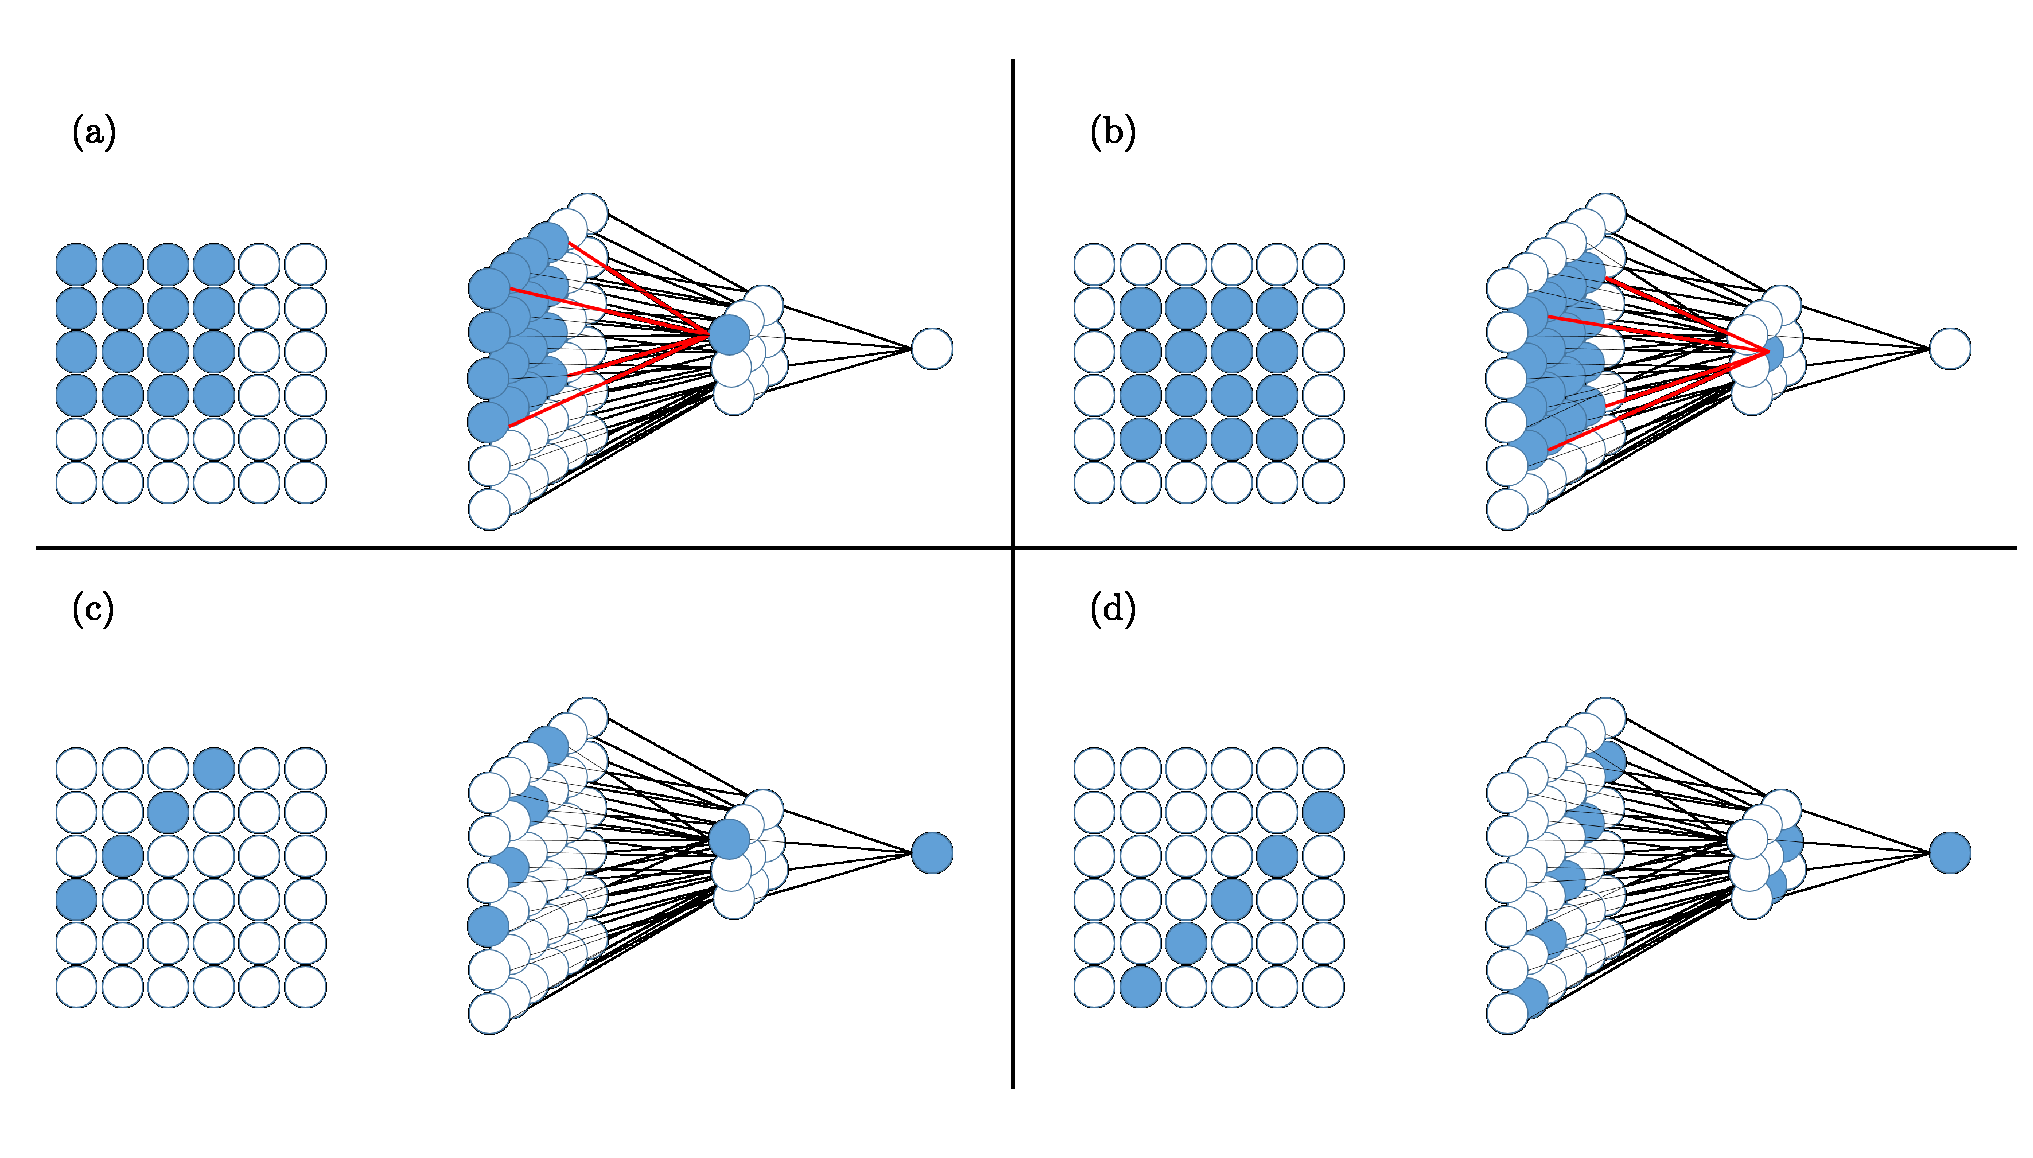
\includegraphics[scale=0.4]{fig/eps/cnn62.eps}
  \caption{単純型細胞と複雑型細胞のモデル}
  \label{fig:単純型細胞と複雑型細胞のモデル}
\end{figure}

\subsection{全体の構造}

\section{プログラム}
\subsection{caffeNetの構造}
caffeでは訓練済みのニューラルネットワークをダウンロードすることができる.先日,示したサンプルの認識に用いたニューラルネットワークの構造をFig.に示す.
\begin{figure}[t]
 \centering
 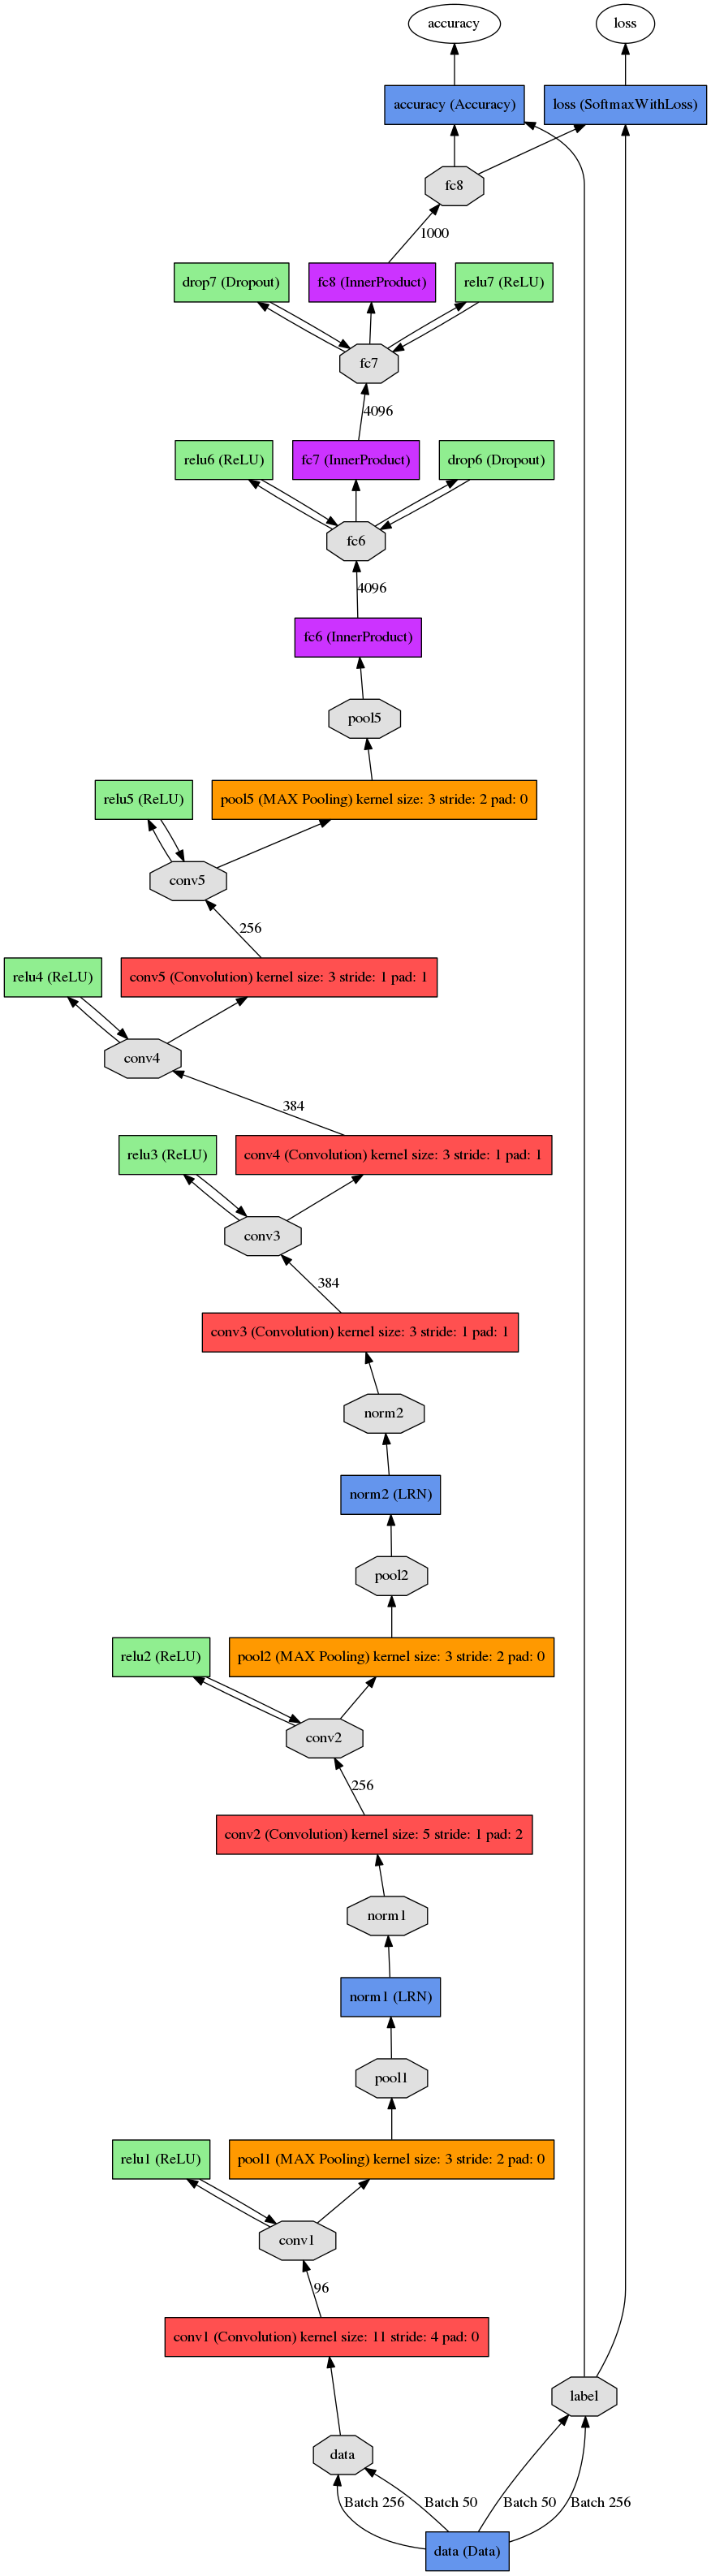
\includegraphics[scale=0.2]{fig/png/caffeNet.png}
  \caption{caffeNet}
\end{figure}

\section{今後の課題}
\begin{itemize}
 \item 理論研究を進める.
 \item Caffeを使いこなす
\end{itemize}

\end{document}